\begin{frame}{The CKM matrix}
    \begin{equation*}
        V_\text{\!CKM} = \begin{pmatrix}
        V_{\!ud} & V_{\!us} & V_{\!ub} \\
        V_{\!cd} & V_{\!cs} & V_{\!cb} \\
        V_{\!td} & V_{\!ts} & V_{\!tb}
        \end{pmatrix} = 
        \underbrace{\begin{pmatrix}
        1 - \sfrac{\textcolor{vertexDarkBlue}{\lambda}^2}{2} & \textcolor{vertexDarkBlue}{\lambda} & A \textcolor{vertexDarkBlue}{\lambda}^3 (\rho - \mathrm{i} \textcolor{vertexDarkRed}{\eta}) \\
        -\textcolor{vertexDarkBlue}{\lambda} & 1 - \sfrac{\textcolor{vertexDarkBlue}{\lambda}^2}{2} & A \textcolor{vertexDarkBlue}{\lambda}^2 \\
        A \textcolor{vertexDarkBlue}{\lambda}^3 (1 - \rho - \mathrm{i} \textcolor{vertexDarkRed}{\eta}) & -A \textcolor{vertexDarkBlue}{\lambda}^2 & 1
        \end{pmatrix}}_{\text{\cf{} Wolfenstein: Phys.\,Rev.\,Lett. 51 (1945), 21}}
        + \mathcal{O}(\textcolor{vertexDarkBlue}{\lambda}^3)
    \end{equation*}
    \hfill{\footnotesize $\textcolor{vertexDarkBlue}{\lambda} \approx .23$, $A \approx .81$, $\rho \approx .14$, $\textcolor{vertexDarkRed}{\eta} \approx .35$}
    \begin{itemize}
        \item \underline{One} non-trivial complex phase, encoded in matrix elements
        \begin{itemize}
            \item $V_{\!ub}$ and $V_{\!td}$ (up to $\mathcal{O}(\textcolor{vertexDarkBlue}{\lambda}^2)$)
            \item $V_{\!cd}$, $V_{\!cs}$ and $V_{\!ts}$ (up to $\mathcal{O}(\textcolor{vertexDarkBlue}{\lambda}^6)$)
        \end{itemize}
        \item CP violation if and only if $\textcolor{vertexDarkRed}{\eta} \neq 0$
    \end{itemize}
\end{frame}

\begin{frame}{The CKM Matrix}
    \begin{columns}[T]
        \begin{column}{.75\textwidth}
            \textbf{CP violation (?)}
            \begin{itemize}
                \item If $\eta \neq 0$ some $V_{\!ij}$ carry a complex phase (\textit{weak} phase)
                \begin{itemize}
                    \item amplitude: $\mathcal{A}(\decay{\tquark}{\dquark \Wp}) \sim V_{\!td}^{\textcolor{vertexDarkRed}{*}}$
                    \item amplitude: $\bar{\mathcal{A}}(\decay{\tquarkbar}{\dquarkbar \Wm}) \sim V_{\!td}$
                    \item CPV since $\mathcal{A} \neq \bar{\mathcal{A}}$ (?)
                \end{itemize}
            \end{itemize}
            \ldots~not quite
            \begin{itemize}
                \item Amplitude $\mathcal{A}$ is not observable \ldots
                \item \ldots~but branching fraction $\mathcal{B} \sim |\mathcal{A}|^2$ is
                \begin{itemize}
                    \item CPV needs at least two interfering decay modes with \ldots
                    \item \ldots\;one \textbf{CP odd} and one \textbf{CP even} phase
                \end{itemize}
            \end{itemize}
        \end{column}
        \begin{column}{.25\textwidth}
            \begin{figure}
                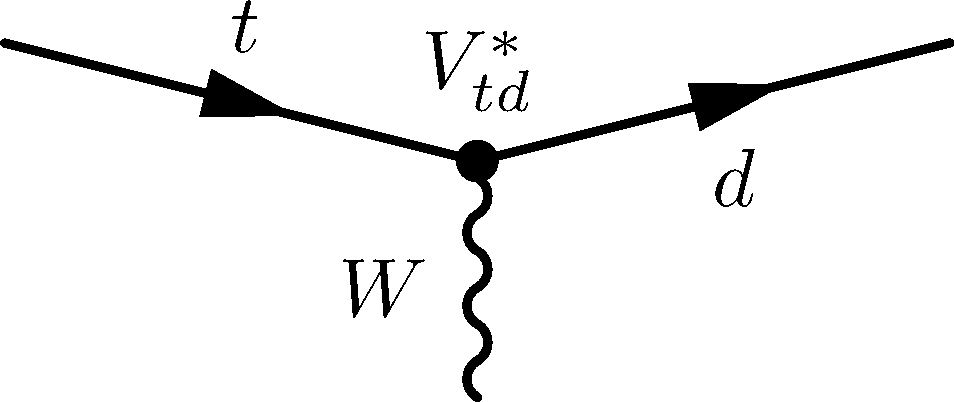
\includegraphics[width=\textwidth]{decay_t2d}
                \caption{\decay{\tquark}{\dquark\Wp}}
            \end{figure}
            \begin{figure}
                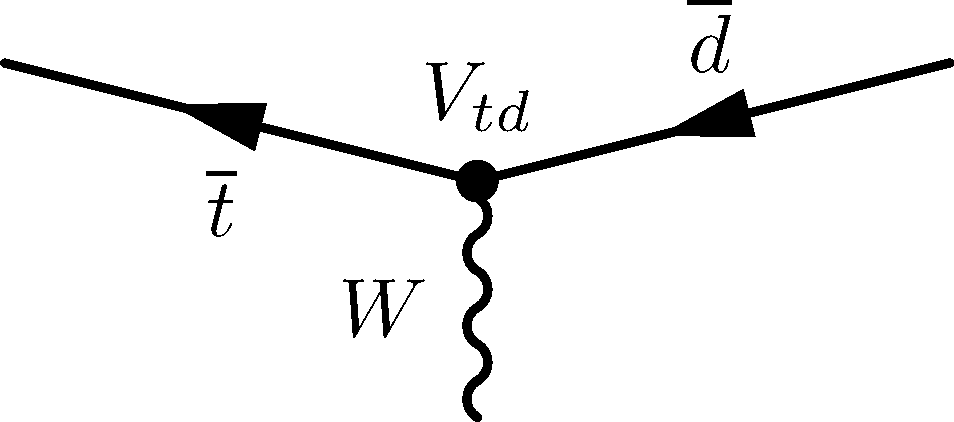
\includegraphics[width=\textwidth]{decay_tb2db}
                \caption{\decay{\tquarkbar}{\dquark\Wm}}
            \end{figure}
        \end{column}
    \end{columns}
\end{frame}

\begin{frame}{Types of CPV}
    \begin{columns}[T]
        \begin{column}{.66\textwidth}
            \begin{column}{.5\textwidth}
                \centering
                \textbf{(1) Direct CPV}
                \begin{equation*}
                    \left| \; 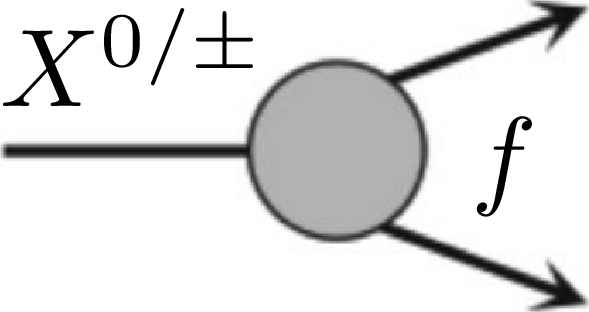
\includegraphics[height=.9cm, valign=c]{cpv1.png} \; \right|^2
                \end{equation*}
                \scalebox{1.5}{$\neq$}
                \begin{equation*}
                    \left| \; 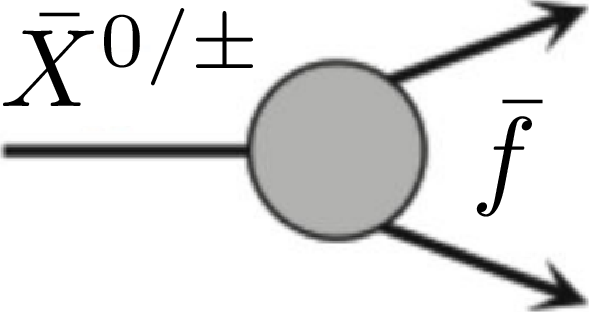
\includegraphics[height=.9cm, valign=c]{cpv1bar.png} \; \right|^2
                \end{equation*}
            \end{column}
            \begin{column}{.5\textwidth}
                \centering
                \textbf{(2) CPV in mixing}
                \begin{equation*}
                    \left| \; 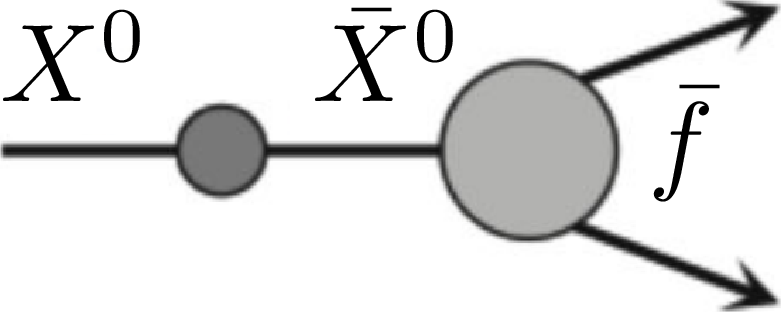
\includegraphics[height=.9cm, valign=c]{cpv2.png} \; \right|^2
                \end{equation*}
                \scalebox{1.5}{$\neq$}
                \begin{equation*}
                    \left| \; 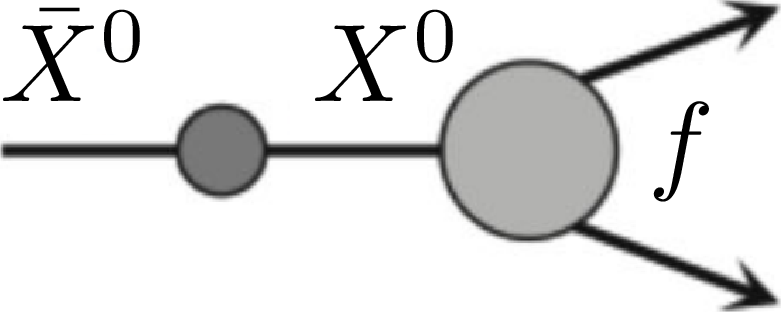
\includegraphics[height=.9cm, valign=c]{cpv2bar.png} \; \right|^2
                \end{equation*}
            \end{column}

            \vspace{5mm}
            \begin{itemize}
                \item CP odd: from CKM matrix
                \item CP even:
                \begin{itemize}
                    \item (1): strong phase difference between both amplitudes (\eg{}, \textit{tree} and \textit{penguin})
                    \item (2), (3): $\pi / 2$ (\textbf{constant!})
                \end{itemize}
            \end{itemize}
        \end{column}
        \begin{column}{.33\textwidth}
            \centering
            \textbf{(3) CPV in interference of mixing and decay}
            \begin{equation*}
                \left| \; 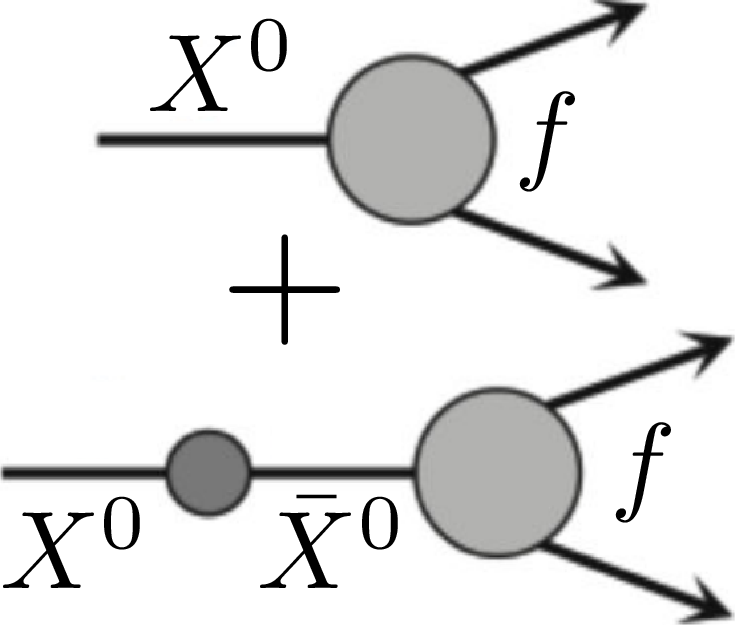
\includegraphics[height=1.8cm, valign=c]{cpv3.png} \; \right|^2
            \end{equation*}
            \scalebox{1.5}{$\neq$}
            \begin{equation*}
                \left| \; 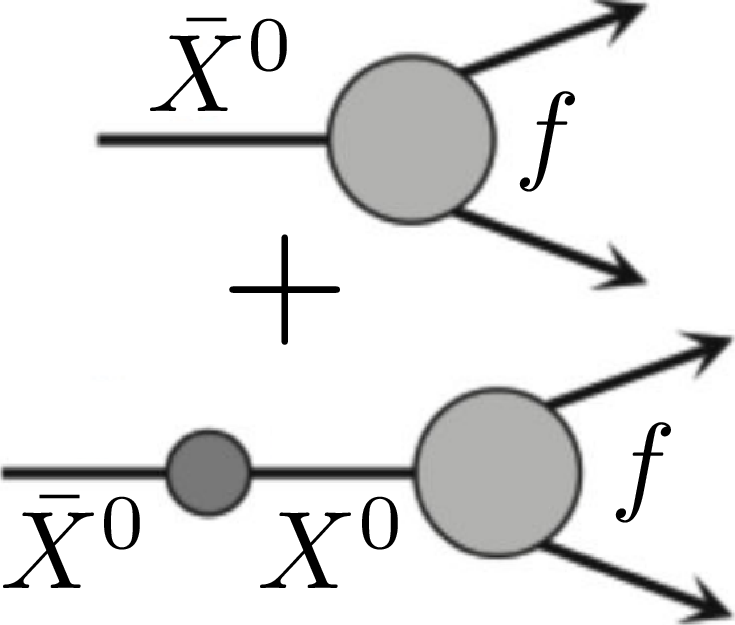
\includegraphics[height=1.8cm, valign=c]{cpv3bar.png} \; \right|^2
            \end{equation*}
            {\tiny \hfill(Images: \textit{CP Violation}, I.\,I. Bigi and A.\,I. Sanda)}
        \end{column}
    \end{columns}
\end{frame}

\begin{frame}{The CKM Matrix}
    \textbf{Another parametrization}
    -- {\footnotesize Prog. Part. Nucl. Phys. 47 (2001)}
    \begin{columns}
        \begin{column}{.7\textwidth}
            \begin{equation*}
                V_\text{\!CKM} = \begin{pmatrix}
                \phantom{-}|V_{\!ud}|\phantom{\mathrm{e}^{-\mathrm{i}\phi_6}} &
                \phantom{-}|V_{\!us}|\phantom{\mathrm{e}^{-\mathrm{i}\phi_6}} &
                \phantom{-}|V_{\!ub}| \mathrm{e}^{-\mathrm{i}\tilde\gamma}\\
                -|V_{\!cd}| \mathrm{e}^{+\mathrm{i}\phi_4} &
                \phantom{-}|V_{\!cs}| \mathrm{e}^{-\mathrm{i}\phi_6} &
                \phantom{-}|V_{\!cb}|\phantom{\mathrm{e}^{-\mathrm{i}\tilde\gamma}} \\
                \phantom{-}|V_{\!td}| \mathrm{e}^{-\mathrm{i}\tilde\beta\phantom{{}_4}} &
                -|V_{\!ts}| \mathrm{e}^{+\mathrm{i}\phi_2} &
                \phantom{-}|V_{\!tb}|\phantom{\mathrm{e}^{-\mathrm{i}\tilde\gamma}}
                \end{pmatrix}
            \end{equation*}
        \end{column}
        \begin{column}{.3\textwidth}
            \scalebox{.75}{\parbox{\linewidth}{%
            \begin{align*}
                &\gamma \equiv \tilde\gamma - \phi_4, & \phi_\mathbf{2} &\approx \eta \textcolor{vertexDarkBlue}{\lambda}^\mathbf{2}\\
                &\beta \equiv \tilde\beta + \phi_4, & \phi_\mathbf{4} &\approx \eta A^2 \textcolor{vertexDarkBlue}{\lambda}^\mathbf{4}\\
                &\alpha \equiv \pi - \beta - \gamma, & \phi_\mathbf{6} &\approx \eta A^4 \textcolor{vertexDarkBlue}{\lambda}^\mathbf{6}\\
                &\beta_s \equiv \phi_s \equiv \phi_2 + \phi_6
            \end{align*}}}
        \end{column}
    \end{columns}
    \vfill
    \begin{columns}[T]
        \begin{column}{.6\textwidth}
            \begin{itemize}
                \item From unitarity: 6 triangles
                \begin{itemize}
                    \item $V_{\!ud} V^*_{\!us} \,+\, V_{\!cd} V^*_{\!cs} \,+\, V_{\!td} V^*_{\!ts} = 0$
                    \item $V_{\!ud} V^*_{\!ub} \,+\, V_{\!cd} V^*_{\!cb} \,+\, V_{\!td} V^*_{\!tb} = 0$
                    \item \ldots~4 more 
                \end{itemize}
                \item Angles $\tilde\alpha$, $\tilde\beta$, $\tilde\gamma$ and $\phi_{2,4,6}$ \textbf{depend on phase convention} (\ie{}, not observable)
                \item Phases of products $V_{\!ij} V_{\!kl} V^*_{\!il} V^*_{kj}$ are \textbf{invariant} and \textbf{observable} (\eg{}, $\alpha$, $\beta$, $\gamma$, \ldots)
            \end{itemize}
        \end{column}
        \begin{column}{.4\textwidth}
            \hfill
            $V_{\!ud} V^*_{\!ub} + V_{\!cd} V^*_{\!cb} + V_{\!td} V^*_{\!tb} = 0$\\
            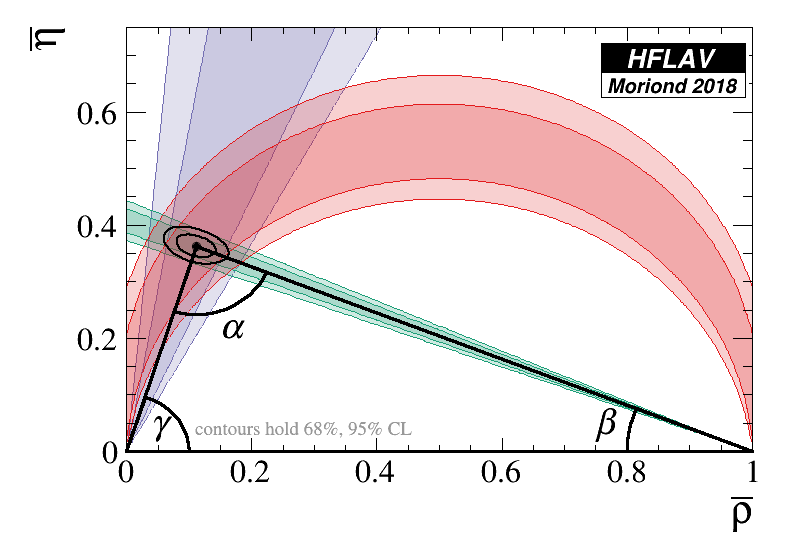
\includegraphics[width=\textwidth]{hflav_rhoeta18}
        \end{column}
    \end{columns}
\end{frame}

\begin{frame}{Probing the SM by Overconstraining}
    \begin{columns}
        \begin{column}{.55\textwidth}
            \begin{itemize}
                \item \textbf{Motivation:}
                \begin{itemize}
                    \item We utterly fail explaining CPV on cosmological scale!
                    \item Is the CKM matrix the only source of CPV?
                    \item Is the SM incomplete / are there more particles?
                \end{itemize}

                \item \textbf{Strategy:}
                \begin{itemize}
                    \item Overconstrain CKM triangles by measuring
                    \begin{itemize}
                        \item sides -- \eg{}, $|V_{\!td} V^*_{\!tb}|$
                        \item angles -- \eg{}, $\gamma = \arg \left( -\frac{V_{\!ud} V^*_{\!ub}}{V_{\!cd} V^*_{\!cb}} \right)$
                    \end{itemize}
                    \item Is $\beta_s = \arg \left( -\frac{V_{\!ts} V^*_{\!tb}}{V_{\!cs} V^*_{\!cb}} \right)$  tiny? ($\mathcal{O}(\textcolor{vertexDarkBlue}{\lambda}^2)$)
                \end{itemize}
            \end{itemize}
        \end{column}
        \begin{column}{.45\textwidth}
            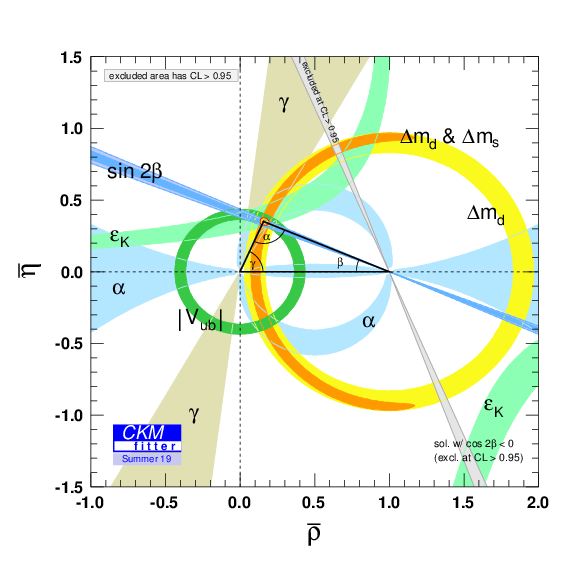
\includegraphics[width=\textwidth]{ckmfitter}
        \end{column}
    \end{columns}

    \centering
    \scalebox{1.2}{Any deviation would point towards \textbf{new physics}, \eg{}, 4th quark family?}
\end{frame}

\begin{frame}{Branching ratios}
    \centering
    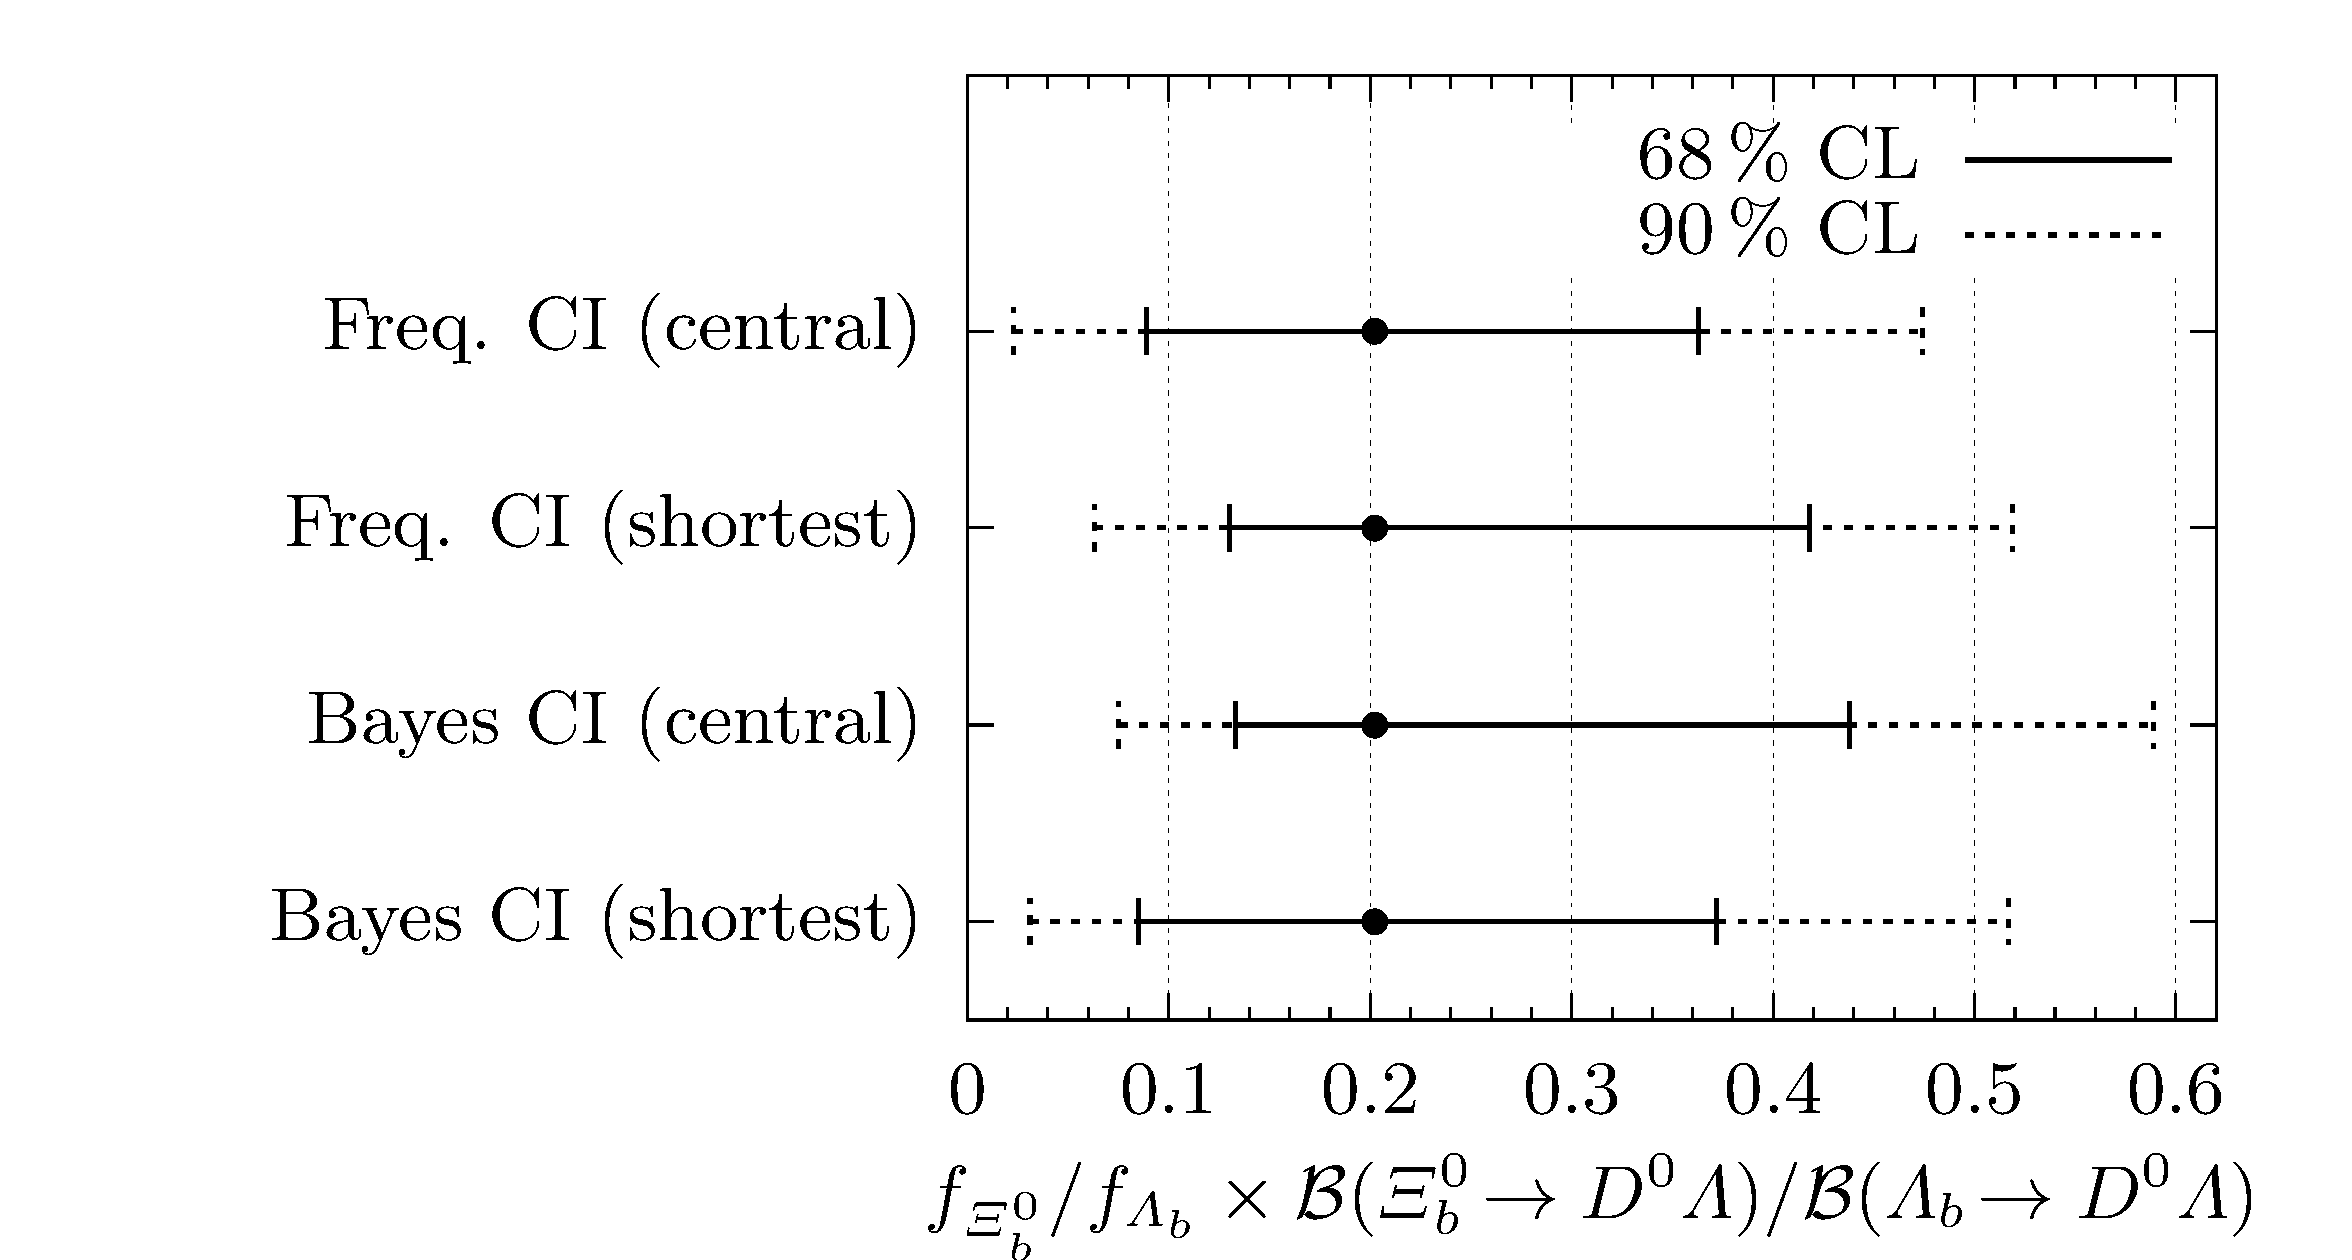
\includegraphics[scale=1.]{br/xiblb_brs.png}
\end{frame}
